\chapter{Foreign visitors' perceptions on Safety Tips.}
\label{c4}

\section{Methodology}
For research objective 1, the data in item 1, item 3, and item 6 shown in Table 1 were used. While considering that the main users of Safety Tips are foreign visitors, only the sample of foreign respondents was selected for this part of the analysis, and the sample of Japanese respondents was excluded in this part. So the total number of samples was 1500.

The first task is to summarize the questionnaire's results from Q15 to Q17. The findings will show the popularity among foreign visitors, past usage experience of foreign respondents, and foreign respondents' perception on Safety Tips in each country, as well as the differences among respondents from the following five countries which are China, South Korea, Indonesia, Thailand, and the UK.

The second task was based on the answers to Q15 and Q16. As Q15 was 'do you know Safety tips or not?', and Q16 was 'Did you use safety tips before or not?', these two questions can clarify respondents' past usage of Safety Tips. The answers to Q15 had three options: Know exactly, Heard safety tips before, and Do not know. If the respondent answered 'Know exactly' or 'Heard Safety tips before', the respondent will continue to answer Q16, if the respondent answers 'Do not know', the respondent will directly skip to Q17. The answers to Q16 are 'used Safety tips before.' and 'never used it before. Therefore, based on the answers to these two questions, all respondents were divided into the following five groups: 'Know exactly and used Safety tips before', 'Know exactly but never used Safety tips before. before', 'Heard Safety tips before and used it before, 'Heard Safety tips before but never used it before, and 'Do not know and never used before. The sample sizes for each group are shown in Figure~\ref{fig6}, which are 'Know exactly and used Safety tips before': 357; 'Know exactly but never used Safety tips before': 90; 'Heard Safety tips before and used it before: 134; 'Heard Safety tips before but never used it before': 465 people; 'Do not know and never used before': 454 people. The results will show whether the two factors of respondents' past awareness and whether they used it before had an impact on their perceptions on Safety Tips.

The third task explored whether demographics and the severity of experienced earthquakes affect respondents' perceptions on Safety Tips. As these variables also may become manifest variables used for SEM, this task also can help us to determine whether the differences in demographic factors and severity of experienced earthquakes will significantly show differences in the responses of "Perception on Safety Tips". We choose the Chi-squared test and Analysis of variance (ANOVA) to finish it.


%%%%%%%%%%%%%%%%%%%%%%%
%\iffalse
\begin{figure*}[h]
  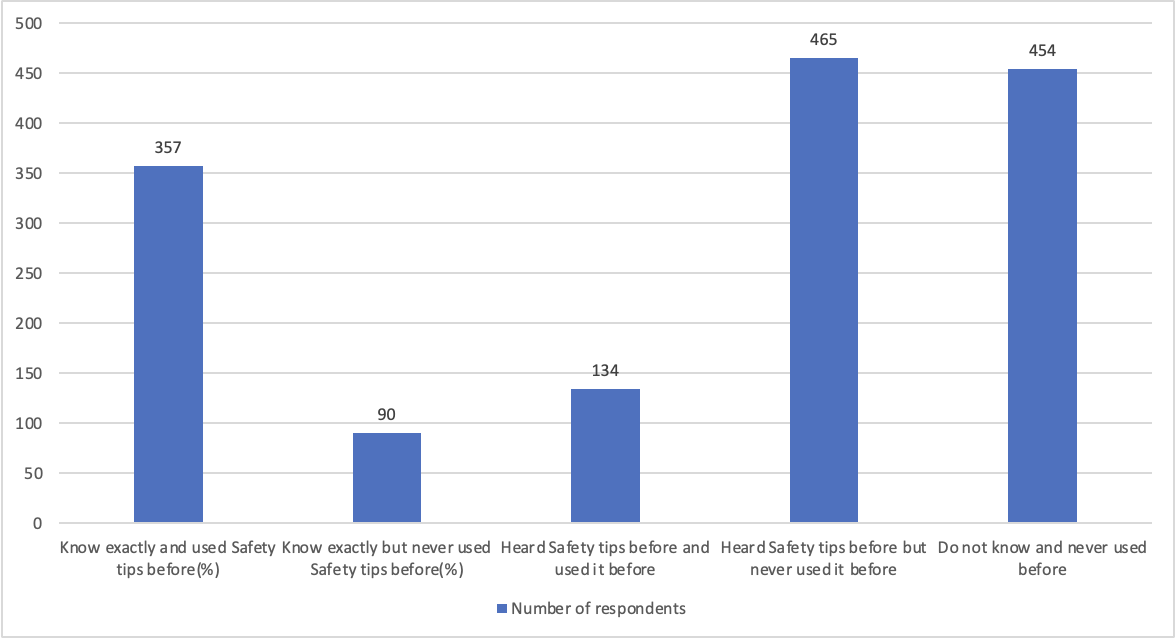
\includegraphics[width=0.7\linewidth]{Figure/Figure6.jpg}
  \centering
  \caption{Number of respondents in each group. }
  \label{fig6}
\end{figure*}
%\fi




\section{Result}

\subsection{Task 1}
For Q15, the result shows in Figure~\ref{fig13}. We can find that around 50\% of the respondents from the UK and Korea do not know Safety Tips before, around 80\% of the respondents from China and Thailand know or at least heard Safety tips before, while around 90\% of the respondents from Indonesia know or at least heard Safety tips before. For Q16, the result shows in Figure~\ref{fig14}. we can find that more than 50\% of the respondents from China, Korea, and Thailand did not use Safety Tips before. Among all countries, respondents from Indonesia have the highest usage rate of Safety Tips at 65.8\%. Koreans had the lowest, at 28\%. 

\begin{figure*}[h]
  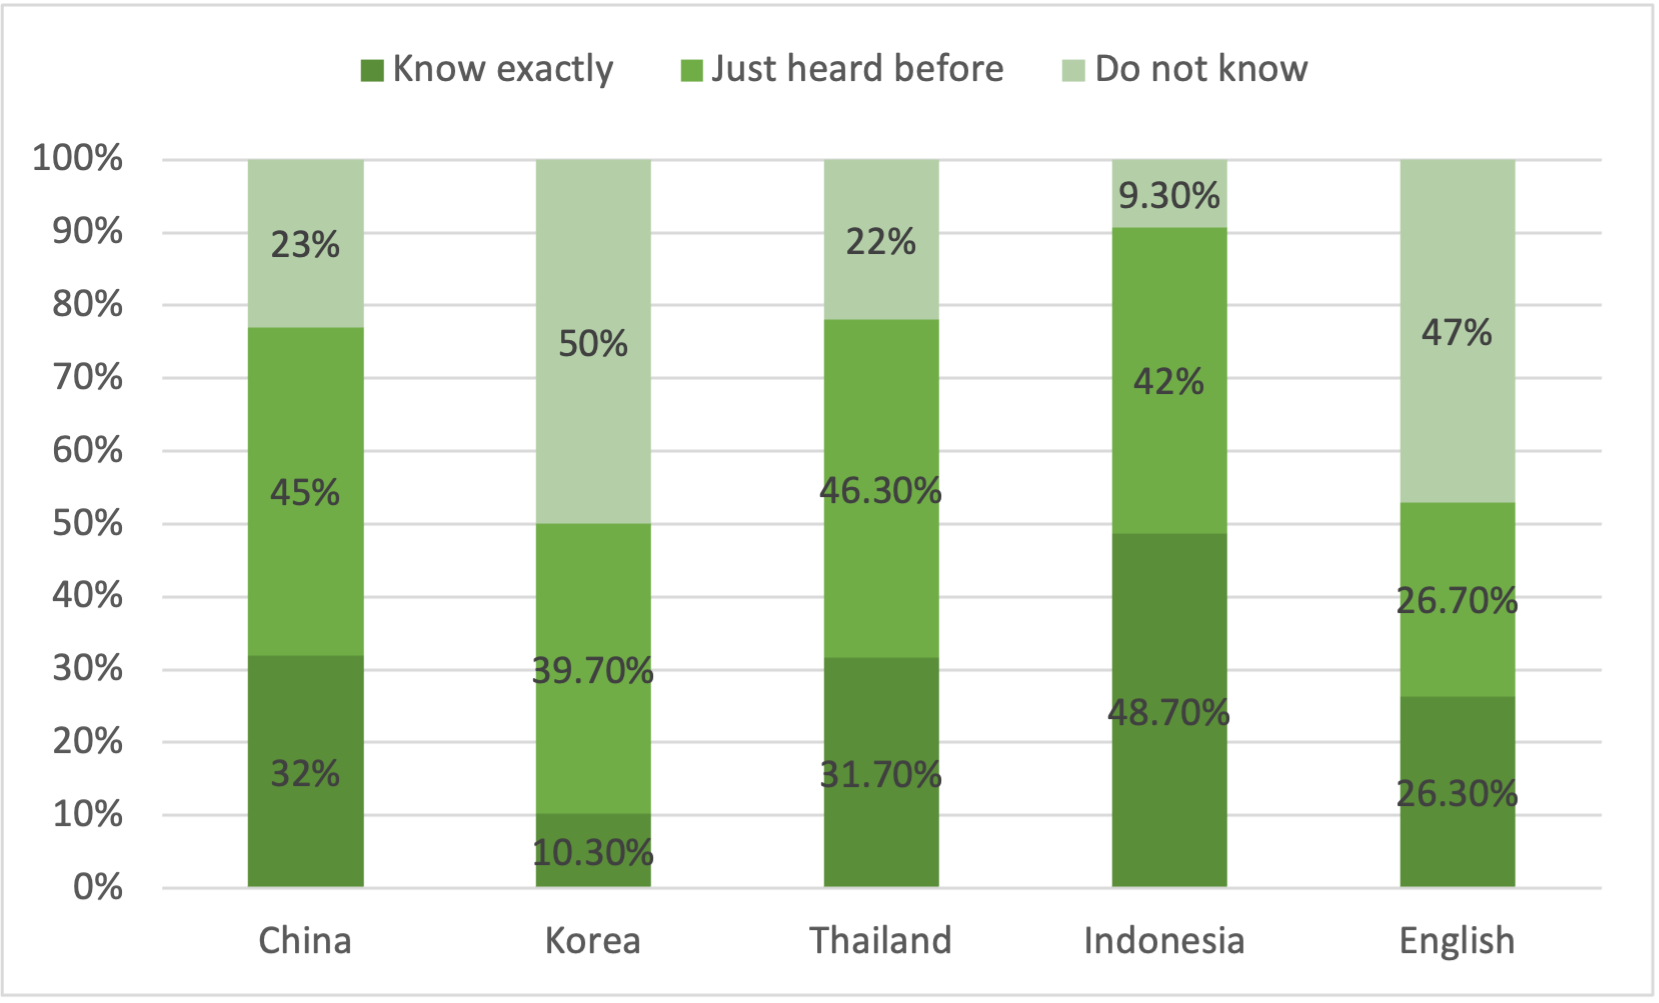
\includegraphics[width=0.6\linewidth]{Figure/Figure13.png}
  \centering
  \caption{Q15: Do you know Safety Tips or not?}
  \label{fig13}
\end{figure*}

\begin{figure*}[h]
  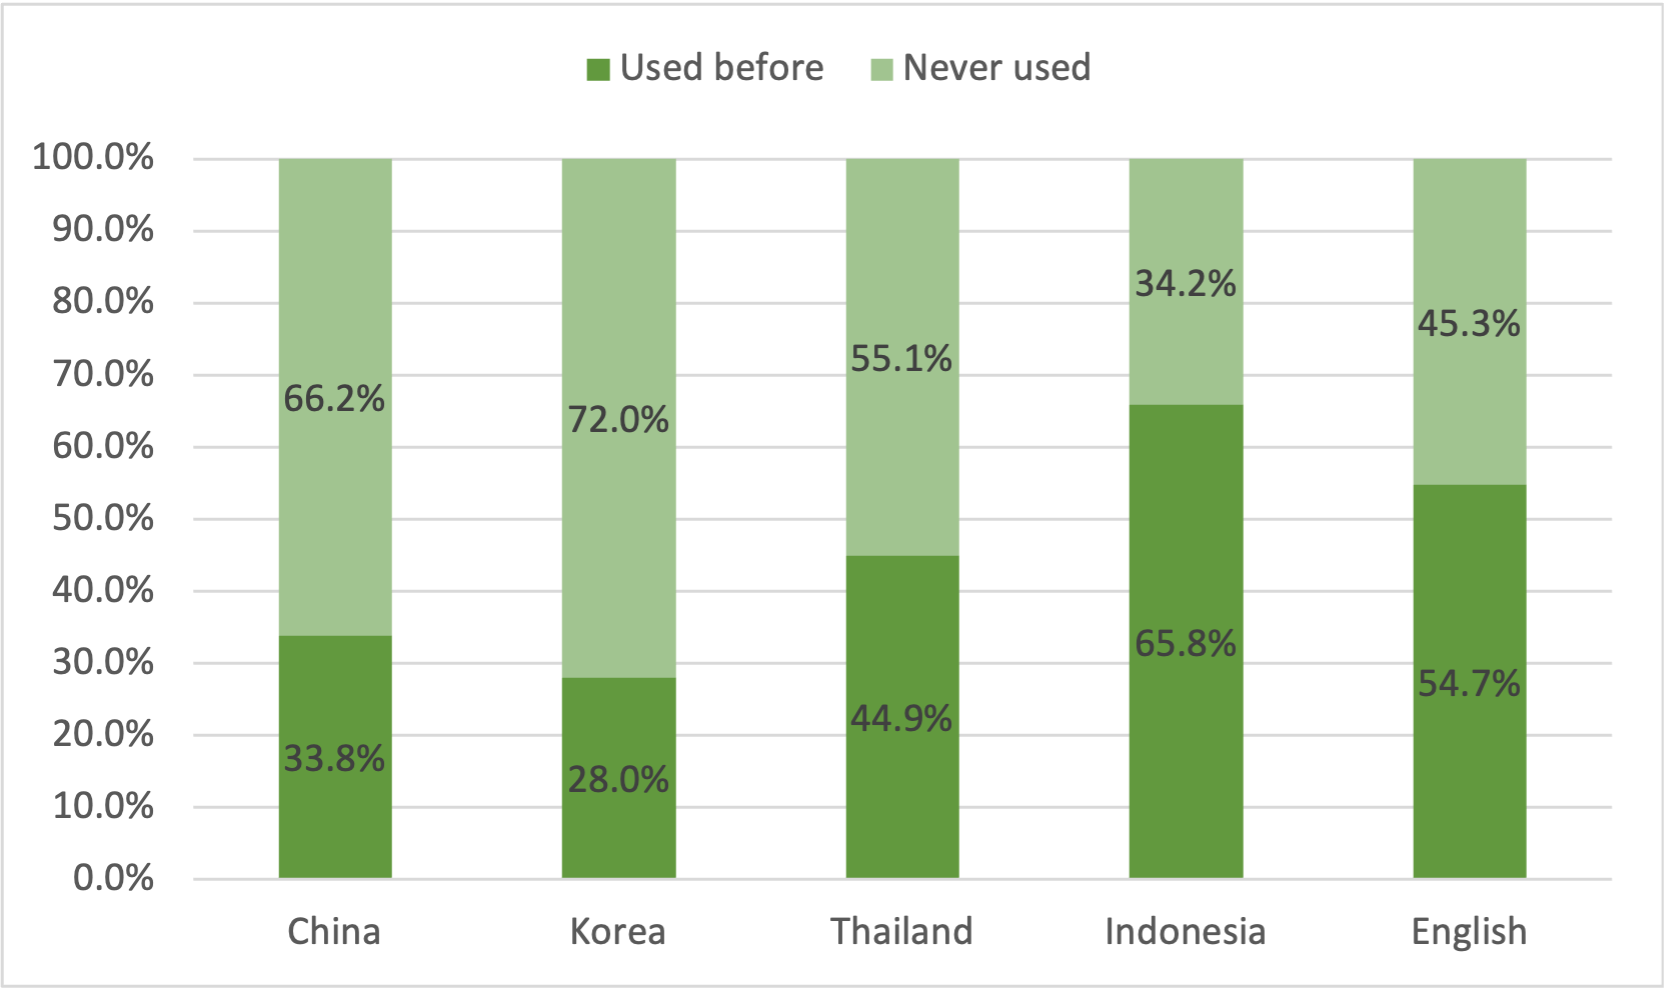
\includegraphics[width=0.6\linewidth]{Figure/Figure14.png}
  \centering
  \caption{Q16: Do you use Safety Tips before or not?}
  \label{fig14}
\end{figure*}

For Q17\_1, the result shows in Figure~\ref{fig15}. We can find that over 90\% of respondents from Thailand and Indonesia said they trusted information from Safety Tips more than their own country's, while respondents from China, the UK, and Korea have a relatively low level of trust, but still around 70\%. For Q17\_2, the result shows in Figure~\ref{fig16}. We can find that over 90\% of respondents from Thailand and Indonesia said they use Safety Tips to search information before their own country's. For Q17\_3, the result shows in Figure~\ref{fig17}. We can find that over 90\% of respondents from Thailand, China, and Indonesia think Safety Tips could be useful during the evacuation. For Q17\_4, the result shows in Figure~\ref{fig18}. we can find that over 90\% of respondents from Thailand, China, and Indonesia think they will use Safety Tips in the future, and more than 80\% of respondents from the UK and Korea think they will use Safety Tips in the future.

\begin{figure*}[h]
  \begin{subfigure}{0.48\textwidth}
  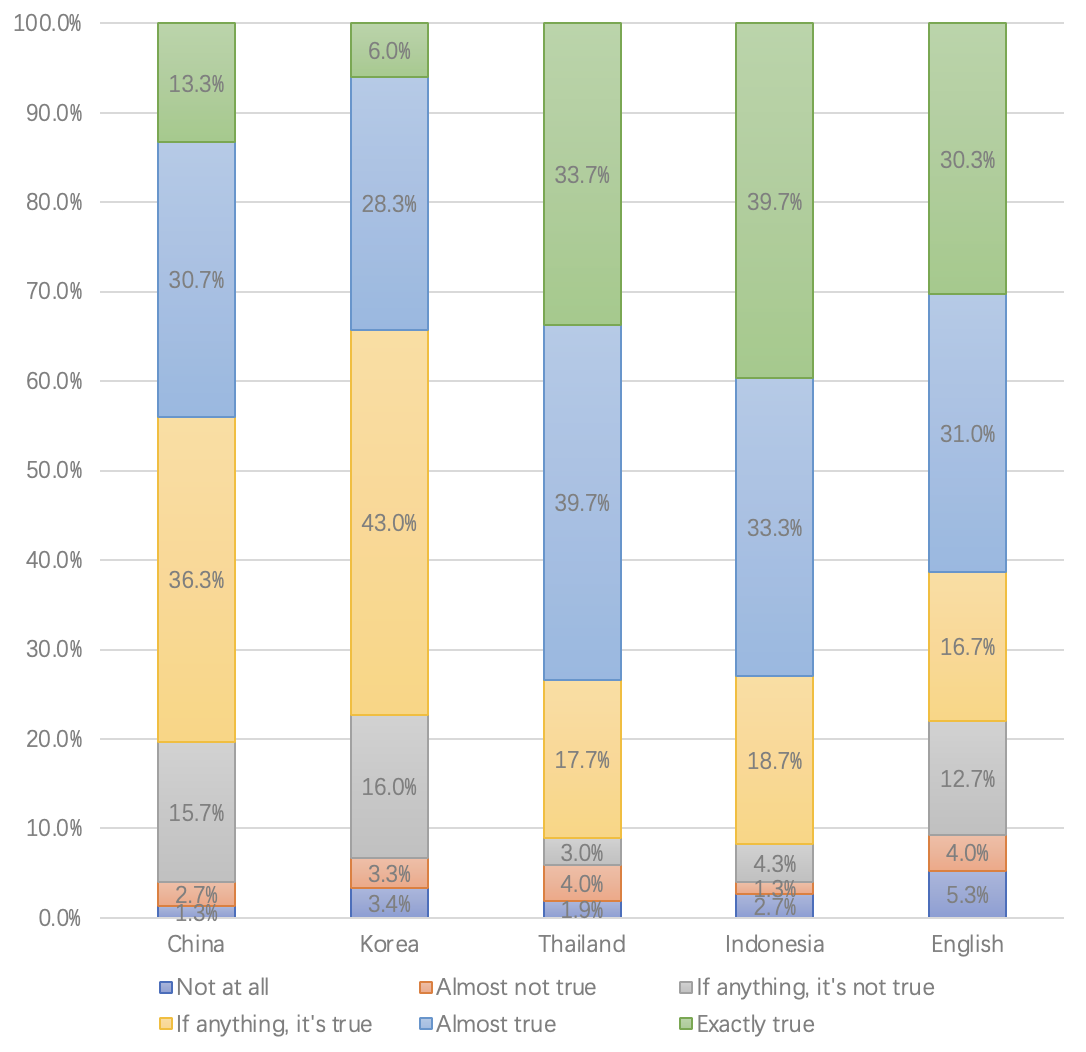
\includegraphics[width=\linewidth]{Figure/Figure15.jpg}
  \centering
  \caption{Q17\_1: Will you trust Safety Tips more than information from your own country?}
  \label{fig15}
  \end{subfigure}\hfill
  \begin{subfigure}{0.48\textwidth}
  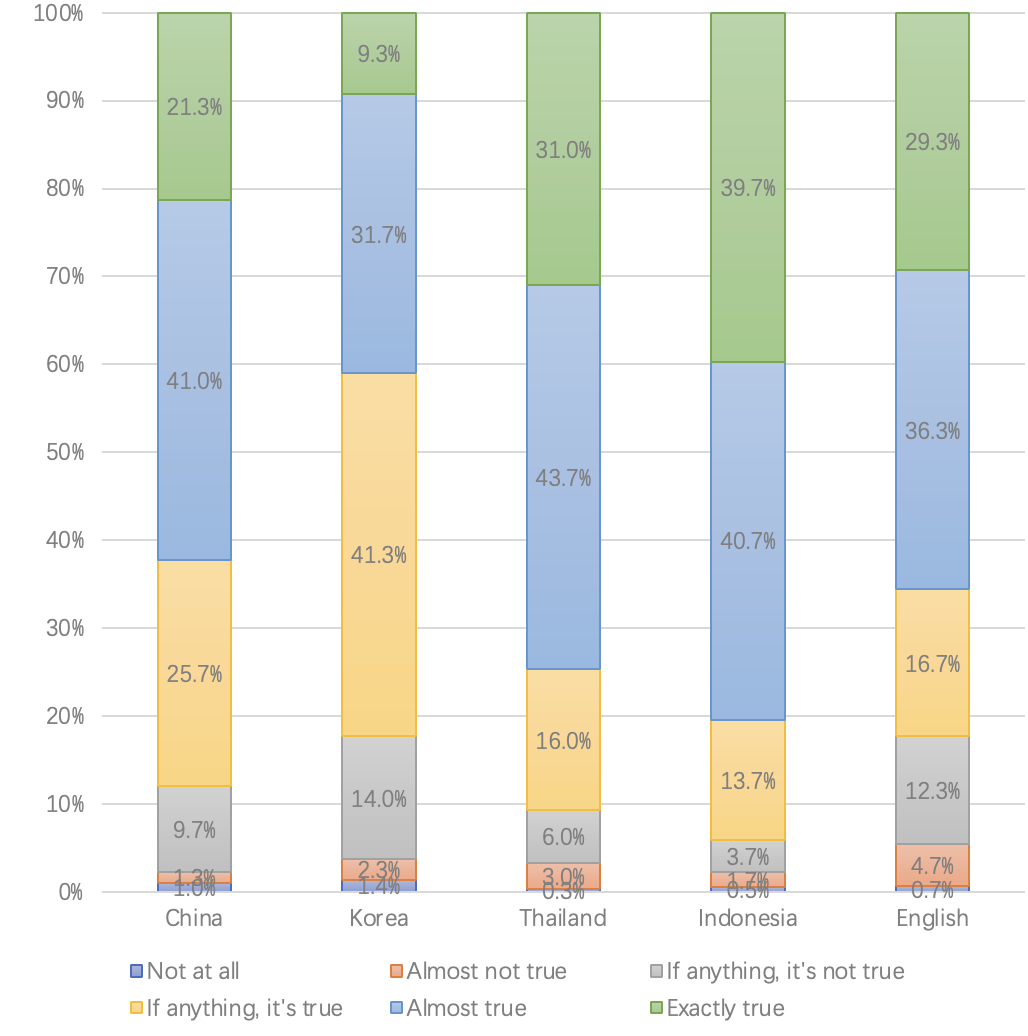
\includegraphics[width=\linewidth]{Figure/Figure16.jpg}
  \centering
  \caption{Q17\_2: Will you use Safety Tips before searching information from your own country?}
  \label{fig16}
  \end{subfigure}
  \begin{subfigure}{0.48\textwidth}
  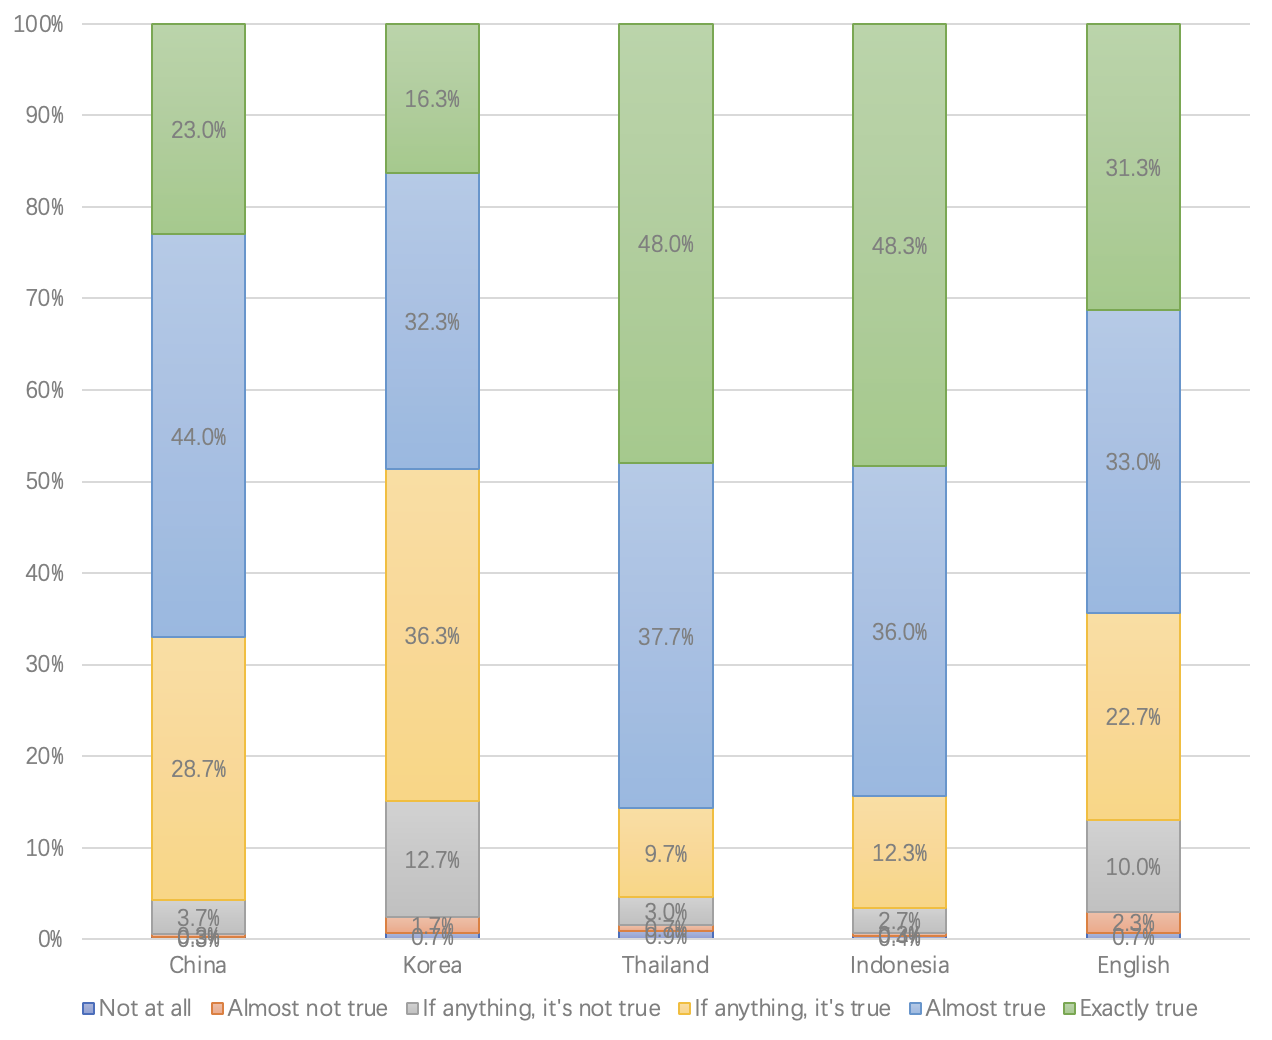
\includegraphics[width=\linewidth]{Figure/Figure17.jpg}
  \centering
  \caption{Q17\_3: Do you think Safety Tips could be useful during evacuation?}
  \label{fig17}
  \end{subfigure}\hfill
  \begin{subfigure}{0.48\textwidth}
  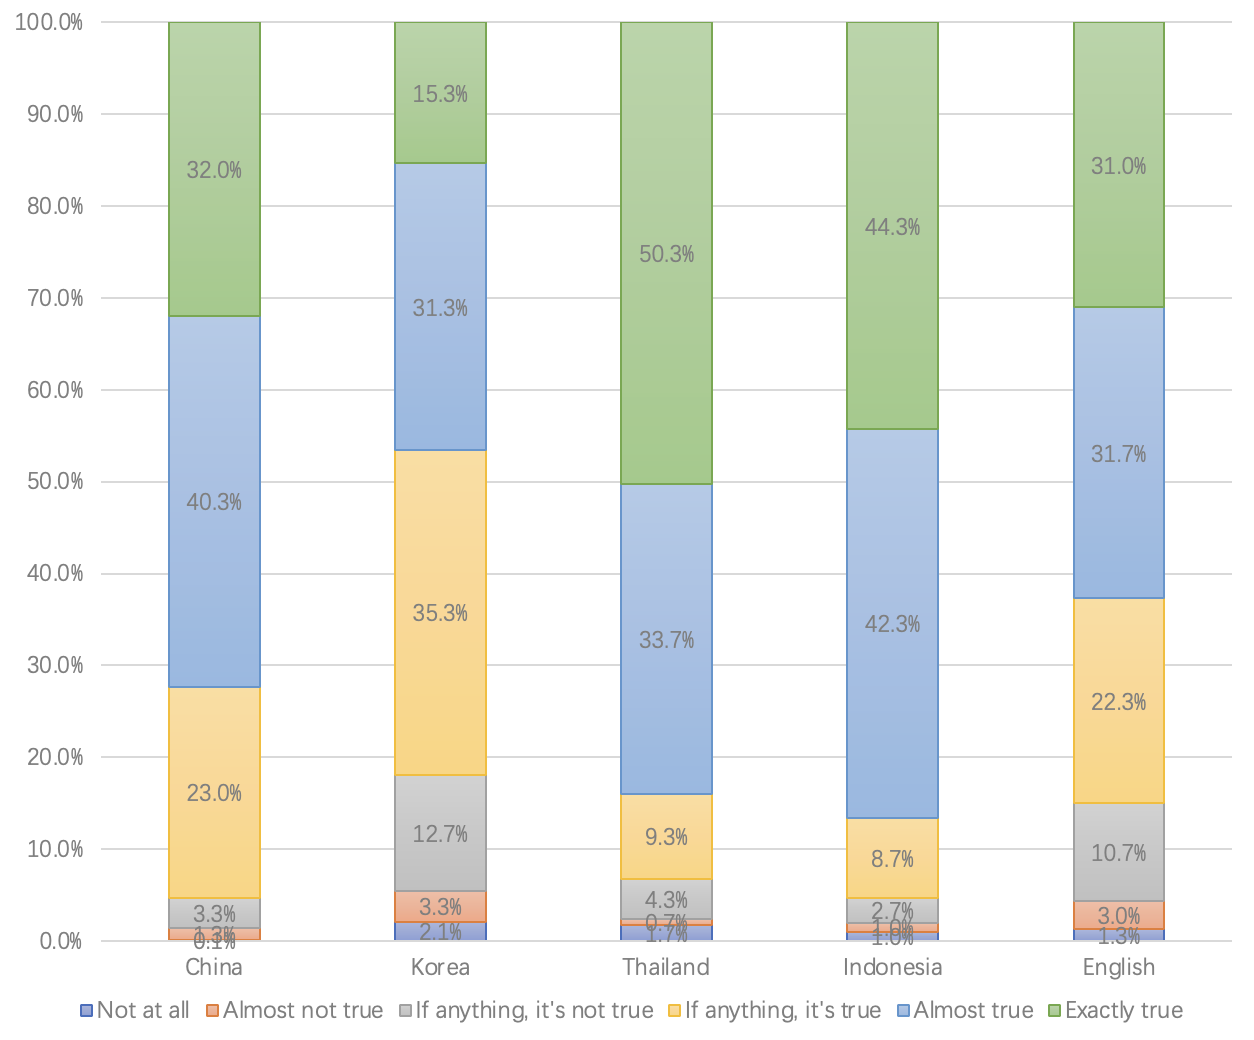
\includegraphics[width=\linewidth]{Figure/Figure18.jpg}
  \centering
  \caption{Q17\_4: Will you use Safety Tips in the future?}
  \label{fig18}
  \end{subfigure}
  \caption{Survey result of perception on Safety Tips}
\end{figure*}



From the above results, we can conclude that from the usage experience, Safety Tips could be more popular and well-known in Indonesia, China, and Thailand than in the UK and Korea. Also, among those respondents that know Safety Tips or heard them before, their usage rate is lower than 70\%. Then from the perception on Safety Tips, we can conclude that over 77\% of the respondents say that they trust Safety Tips more than information from their own countries, over 82\% of the respondents say that they will use Safety tips to search information before from their own countries, and over 84\% of the respondents say that they believe Safety tips could be useful during evacuation and will use Safety tips in the future.

\cleardoublepage
\subsection{Task 2}
In Q15, the question is 'Do you know Safety tips or not?', which asked about respondents' awareness of Safety Tips. And in Q16, the question is 'Did you use Safety tips before or not?', which asked about respondents' past usage experience of Safety Tips. Therefore, in the second task, we aim to find whether the two factors of respondents' awareness and past usage experience had an impact on their attitudes toward Safety Tips. After dividing all respondents into 5 groups, we can find the differences between groups. 

First, from the results of the grouping, we can see that 80\% of those who know Safety Tips have used Safety Tips before. For those who had only heard of Safety Tips, only 22\% of the respondents had used Safety Tips before. Comparing the two sets of data, it is clear that the usage rate has decreased significantly.

For Q17\_1, Will the respondents trust Safety Tips more than information from their country, the result shows in Figure~\ref{fig19}. we can find that respondents who know exactly and used Safety Tips before have shown the highest trust toward Safety Tips, as more than 75\% of the respondents said they trust the information on Safety Tips rather than from their own countries. Respondents who know exactly but never used Safety Tips before and respondents who heard Safety Tips before but never used Safety Tips before are more likely to trust the information on Safety Tips. Respondents who heard and used Safety Tips before and respondents who do not know and never used this application before have shown a relatively negative perception on Safety Tips. 

\begin{figure*}[h]
  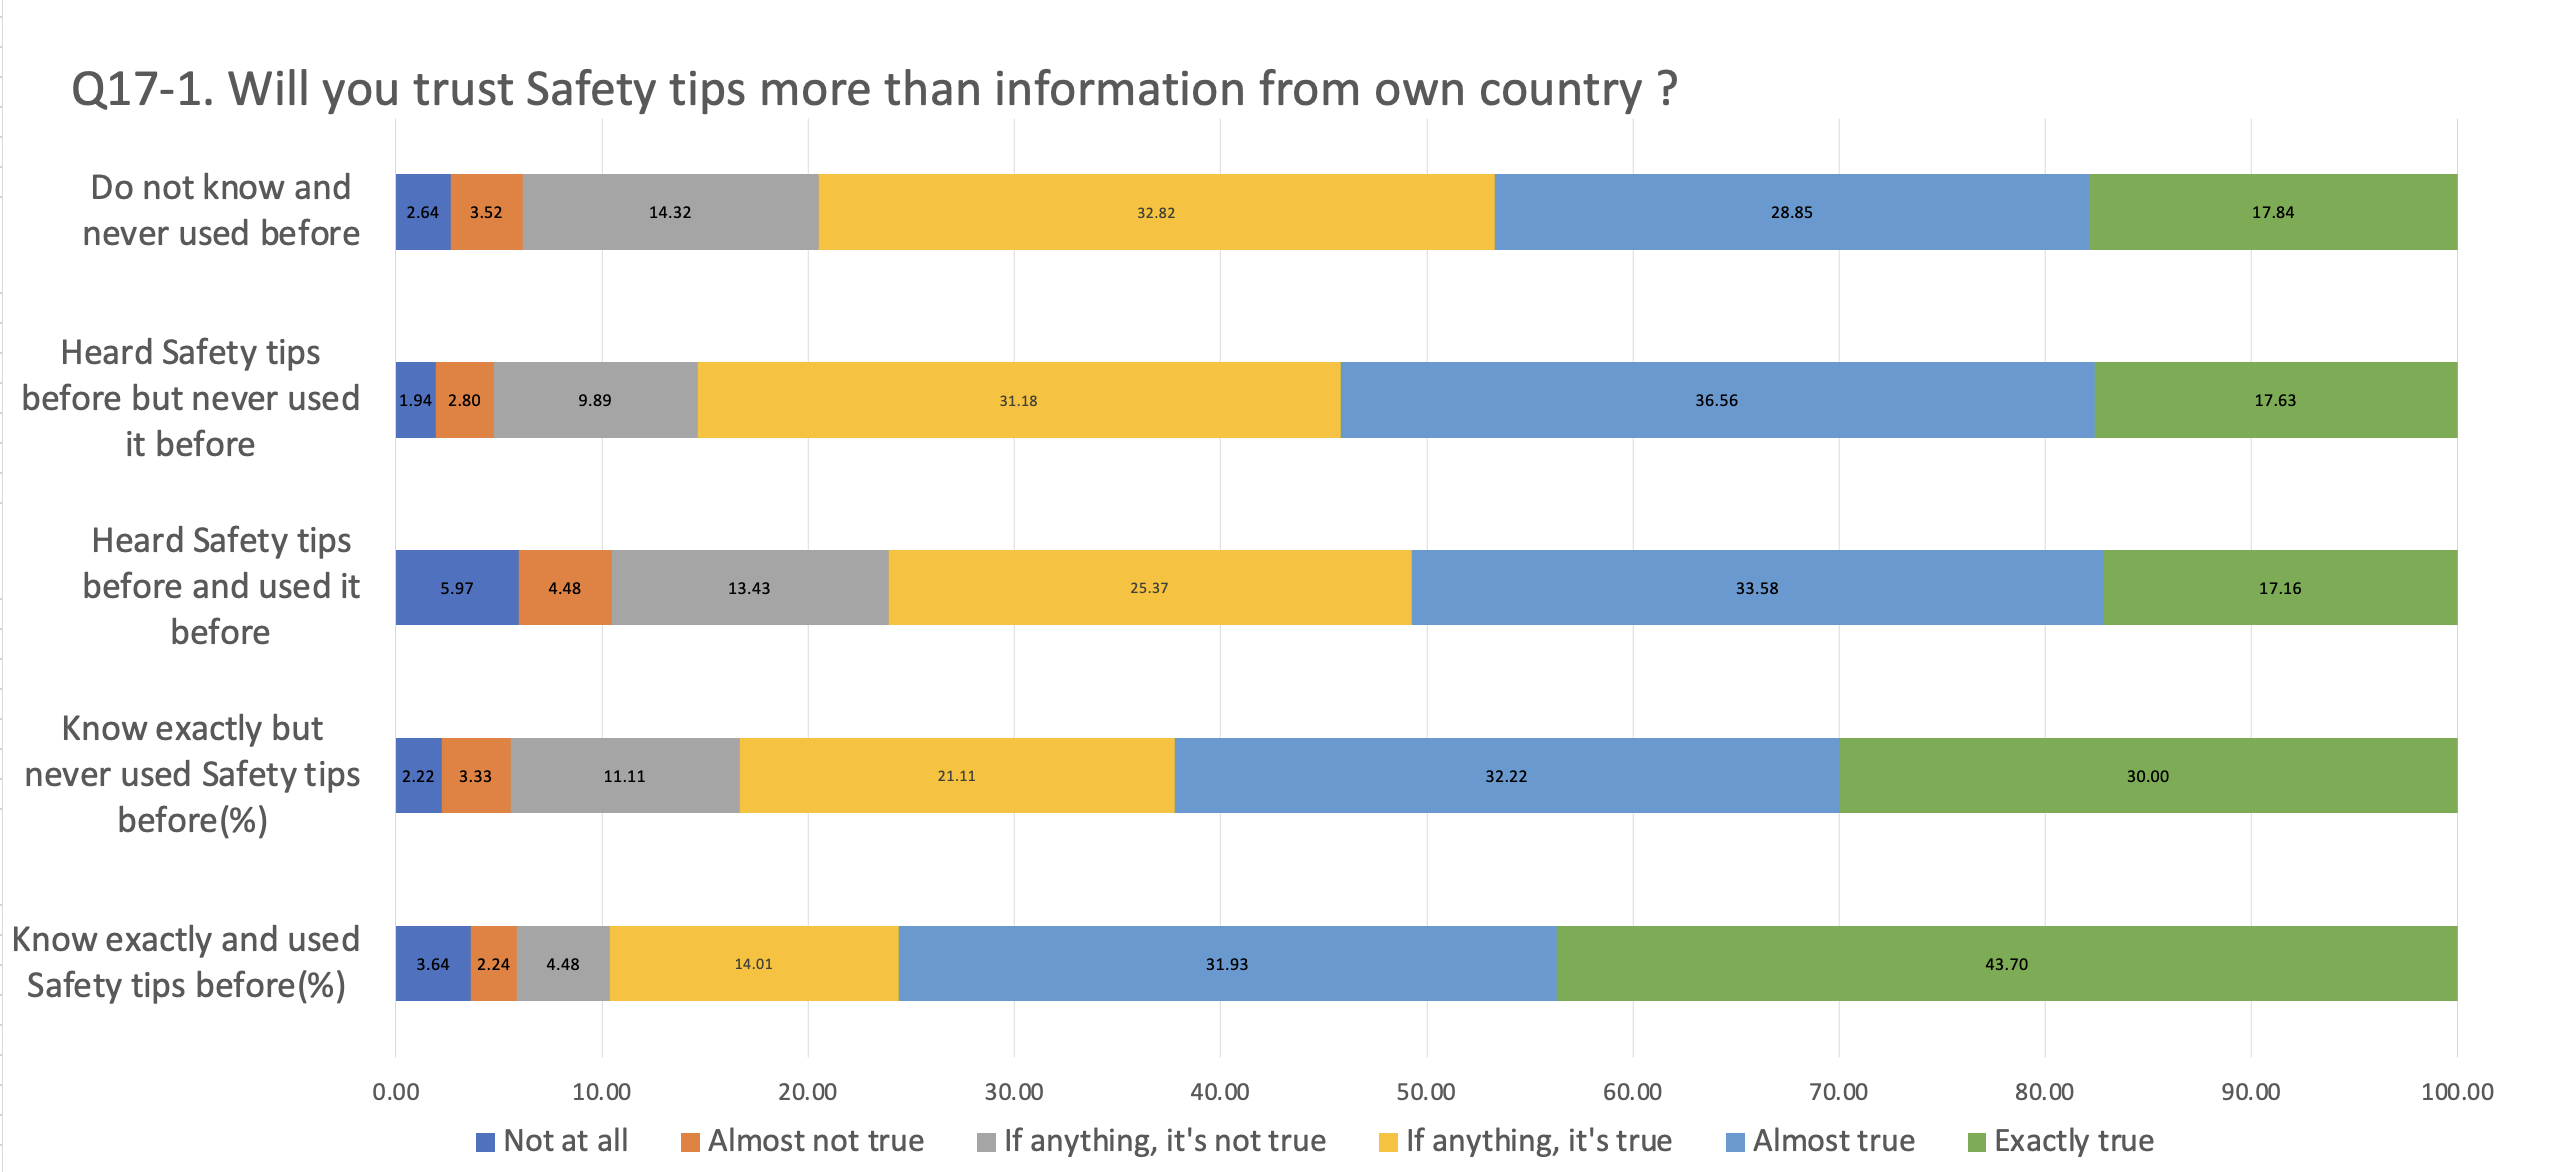
\includegraphics[width=0.8\linewidth]{Figure/Figure19.jpg}
  \centering
  \caption[5 groups of respondents' survey result of Q17\_1]{5 groups of respondents' survey result of Q17\_1(Will you trust Safety Tips more than information from your own country ?)}
  \label{fig19}
\end{figure*}

For Q17\_2, Will the respondents use Safety Tips before searching information from their country, the result shows in Figure~\ref{fig20}. we can find that the respondents who know exactly and used Safety Tips before have shown the highest usage possibility on Safety Tips, as more than 80\% of the respondents said Safety Tips have a higher priority of usage rather than from their own countries. Respondents that know exactly but never used Safety Tips before and respondents who heard Safety Tips before but never used Safety Tips before have shown similar perceptions on the priority of using Safety Tips. Respondents who do not know and never used before and respondents who heard Safety Tips before and used Safety Tips before have shown a little bit lower usage priority. 

\begin{figure*}[h]
  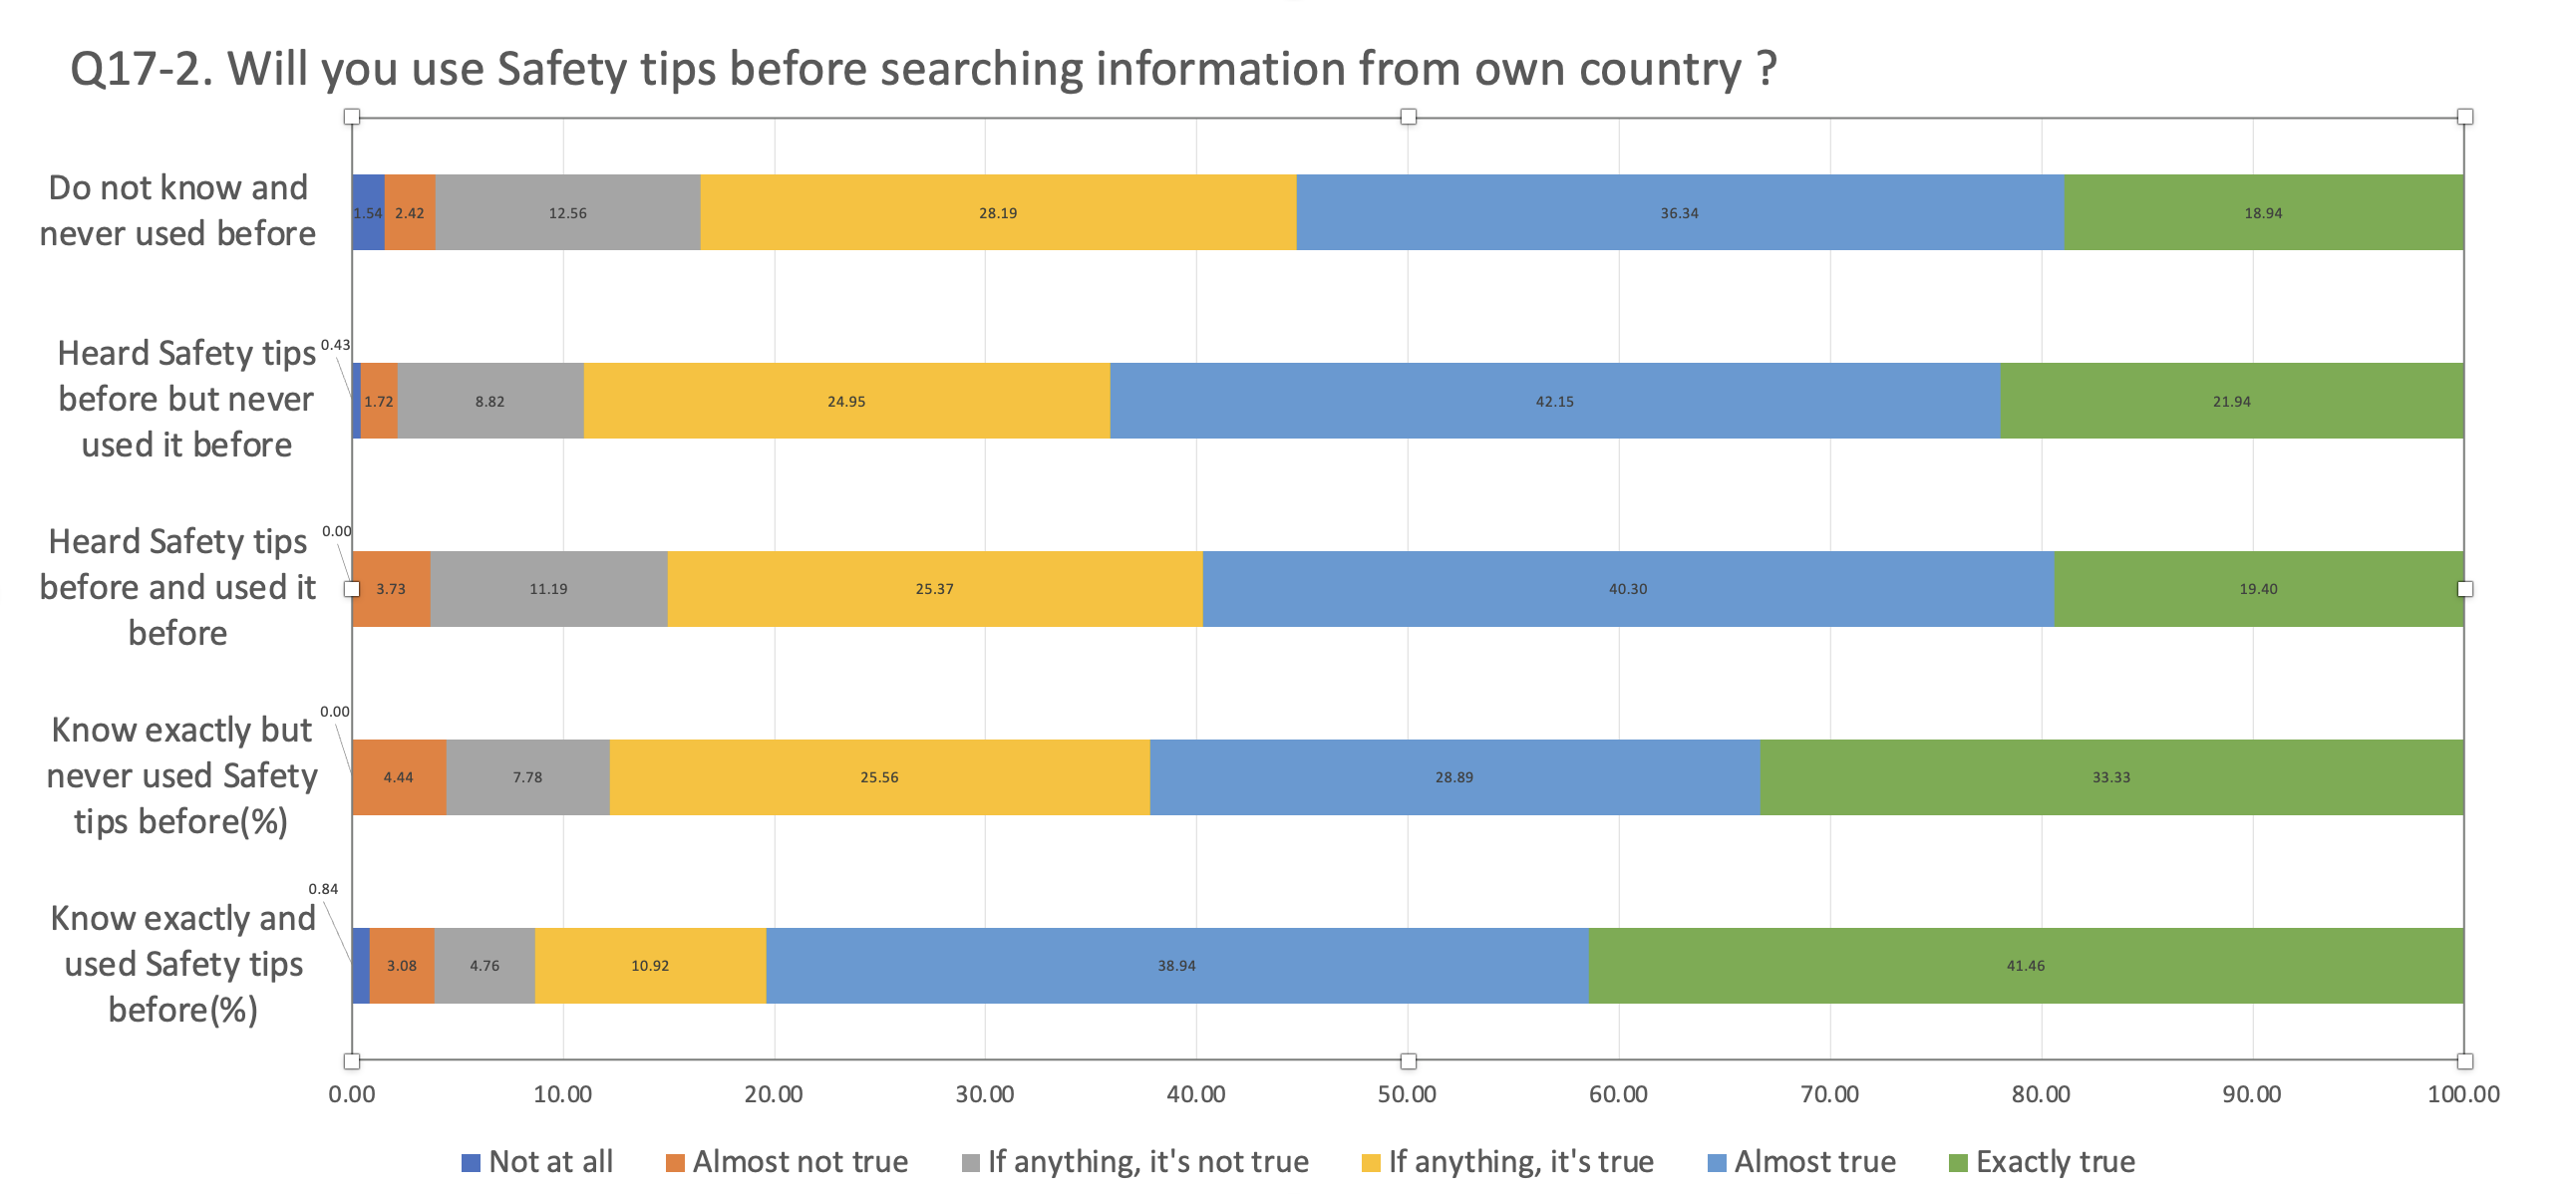
\includegraphics[width=0.8\linewidth]{Figure/Figure20.jpg}
  \centering
  \caption[5 groups of respondents' survey result of Q17\_2]{5 groups of respondents' survey result of Q17\_2(Will you use Safety Tips before searching information from your own country ?)}
  \label{fig20}
\end{figure*}

For Q17\_3, do the respondents think Safety Tips could be useful during the evacuation, the result is shown in Figure~\ref{fig21}. we can find that respondents that know exactly and used Safety Tips before and respondents who heard Safety Tips before but never used Safety Tips before could be more likely to believe Safety Tips could be useful during evacuation. Respondents that do not know and never used before, respondents who heard and used Safety Tips before, respondents who know exactly but never used Safety Tips before could be more likely to show lower usefulness of Safety Tips. 

\begin{figure*}[h]
  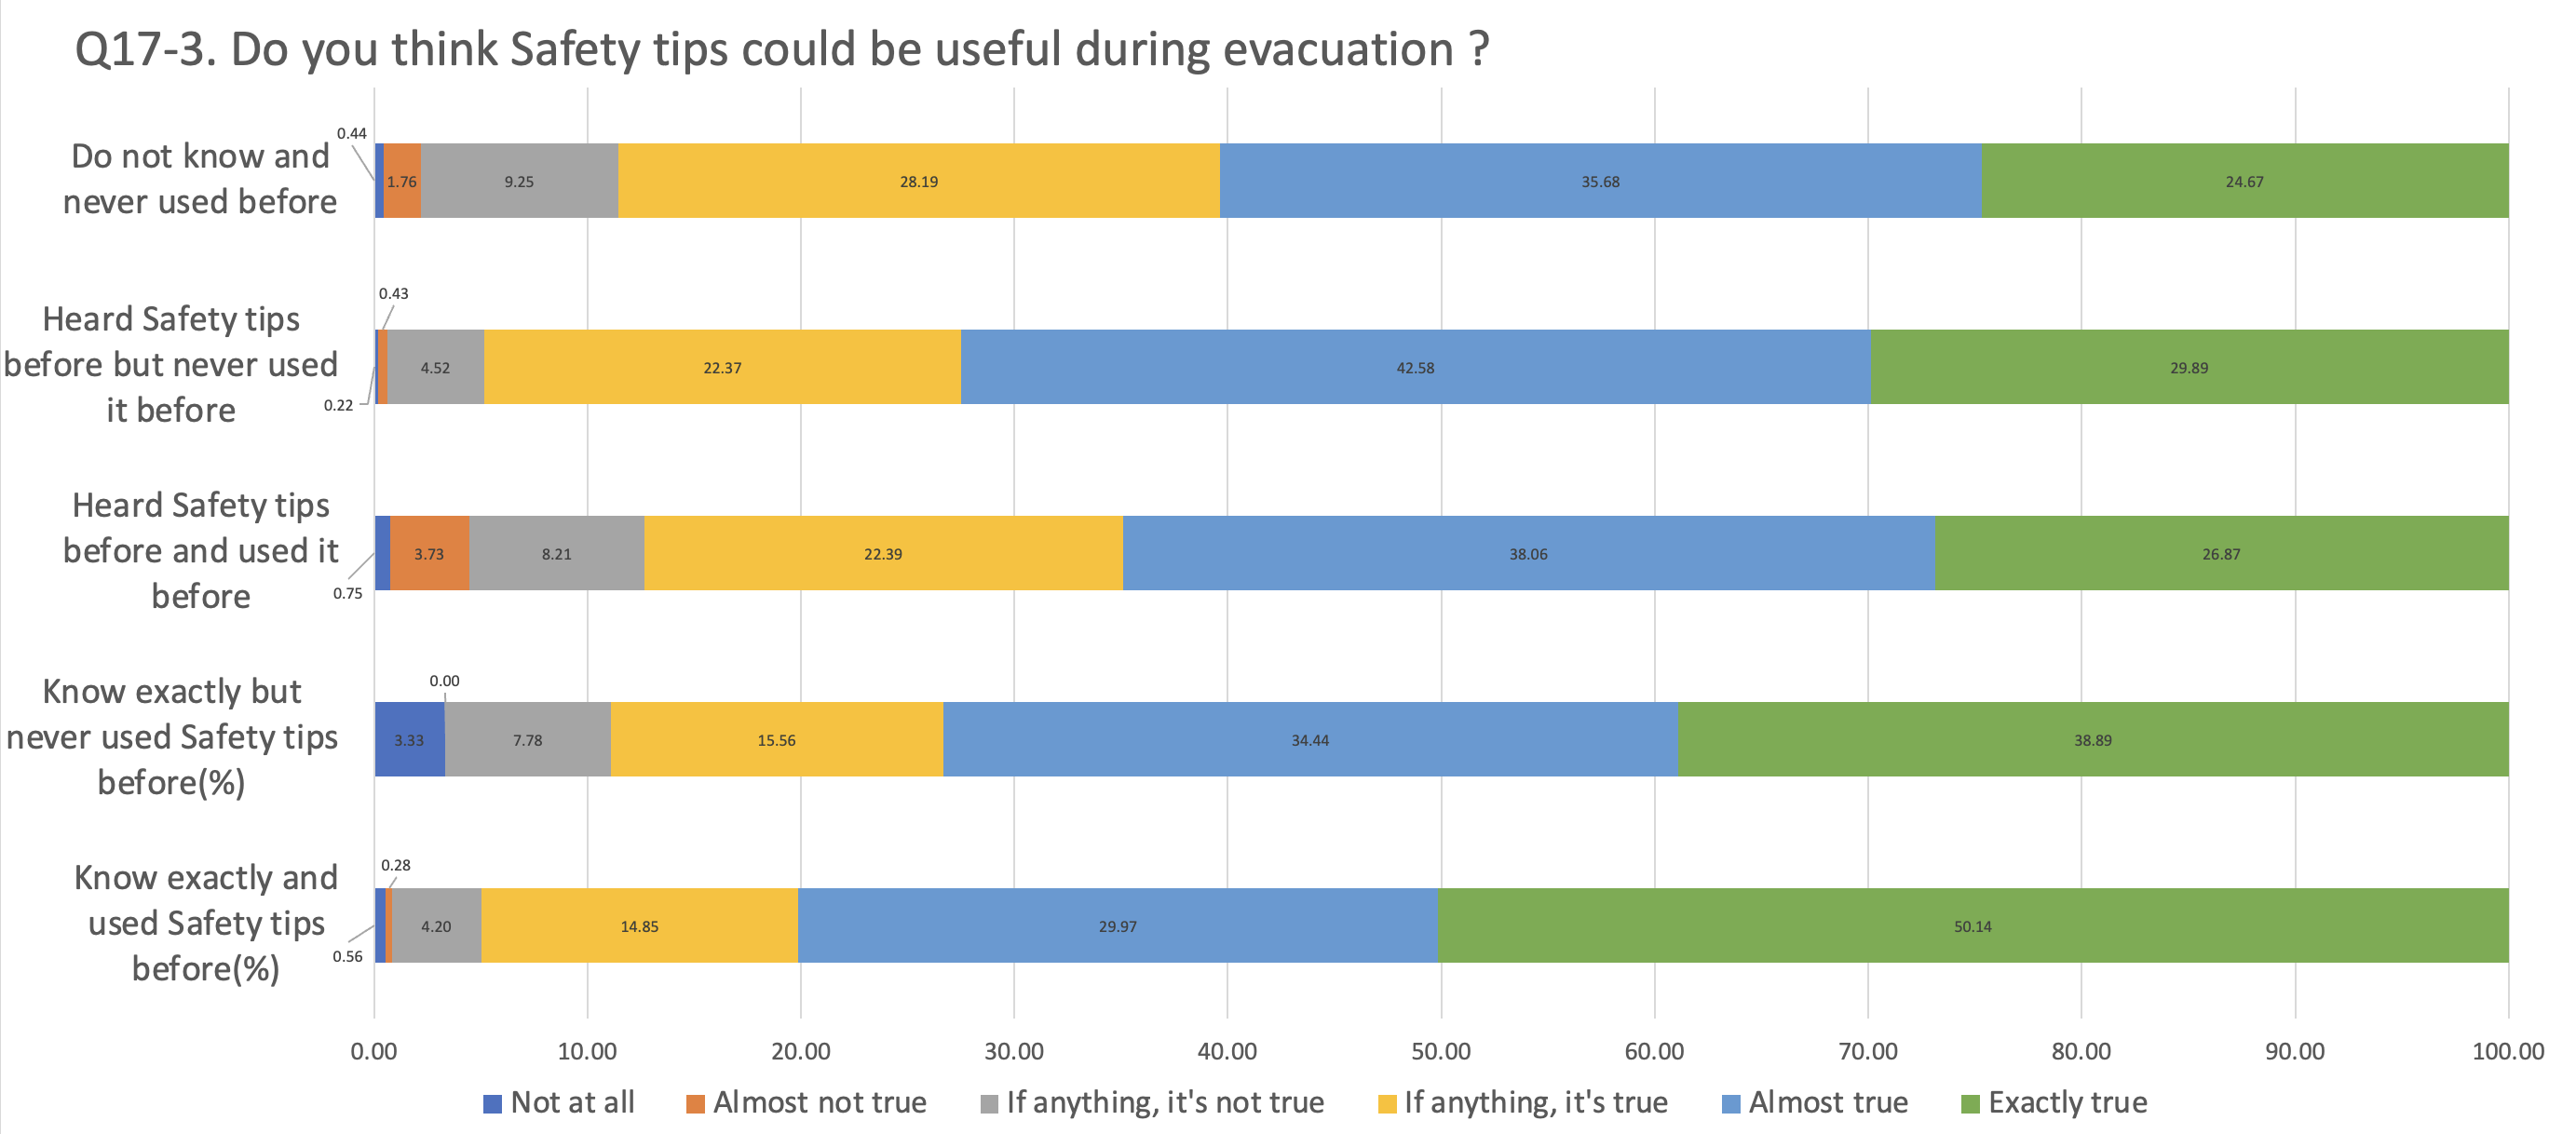
\includegraphics[width=0.8\linewidth]{Figure/Figure21.jpg}
  \centering
  \caption[5 groups of respondents' survey result of Q17\_3]{5 groups of respondents' survey result of Q17\_3(Do you think Safety Tips could be useful during evacuation ?)}
  \label{fig21}
\end{figure*}

For Q17\_4, will the respondents use Safety Tips in the future, the result shows in Figure~\ref{fig22}. we can find that respondents that know exactly and used Safety Tips before and respondents who heard but never used Safety Tips before have shown higher usage possibly Safety Tips in the future. Respondents that do not know and never used before, respondents who heard and used Safety Tips before, respondents who know exactly but never used Safety Tips before have shown relatively lower usage possibility.

\begin{figure*}[h]
  \includegraphics[width=0.8\linewidth]{Figure/Figure22.jpg}
  \centering
  \caption[5 groups of respondents' survey result of Q17\_4]{5 groups of respondents' survey result of Q17\_4(Will you use Safety Tips in the future ?)}
  \label{fig22}
\end{figure*}

From the above results, we can conclude that respondents that know exactly and used Safety Tips before could show higher trust and higher priority of use on Safety Tips, also they are more likely to believe Safety Tips can be useful during the evacuation, and they will use it in the future. And, respondents that heard but never used  Safety Tips before have shown better perceptions on Safety Tips rather than respondents who do not know and never used  Safety Tips before, respondents who heard and used Safety Tips before, respondents who know exactly but never used it Safety Tips before.

The results of the grouping indicate that 80\% of those who clearly know Safety Tips have actually used Safety Tips before. For those who had only heard of Safety Tips, only 22\% of the respondents had used Safety Tips before. Comparing the two sets of data, it is clear that the usage rate has decreased significantly. This shows that people who have a more detailed awareness of Safety Tips are more likely to use this application, so if we want to increase the usage of Safety Tips, it would be helpful to increase foreign visitors' awareness of this application.

\subsection{Task 3}
\label{task3}
For the scale questions in the questionnaire, we conducted a one-sample t-test, which is a method to test whether there is a difference between the mean of a group and a particular value. Thus, these results can indicate whether people have clear attitudes in their responses to these questions. For question Q17 about the attitude toward Safety Tips, the answers to the scale questions were divided into 6 dimensions, answers are from 1 to 6 meaning not at all applicable, mostly not applicable, somewhat not applicable, somewhat agree, mostly agree, strongly agree. here we can consider 1 to 3 as a negative attitude, and 4 to 6 as a positive attitude, therefor we can set the average value of 3.5 as the test value. Table~\ref{table29} shows the results of the one-sample t-test. For Q17\_1 to Q17\_1, the mean values of 491 respondents are 4.80$\pm$1.31; 4.95$\pm$1.08; 5.10$\pm$1.01; 5.11$\pm$1.02; All of the p values are less than 0.01, mean all are statistically significant at $p<0.001$ level. Compared to the test value of 3.5, indicating that all have significant differences in the perception on Safety Tips, all mean values are higher than the test value of 3.5, implying that respondents show positive perceptions to all of the questions about Safety Tips. 

\begin{table}[h]
  \caption[Result of one-sample t-test]{Result of one-sample t-test (N=491)}
  \label{table29}
  \centering
  \begin{tabular}{l|cccc}
 \hline
                  & Mean                 & Test Value & t                          & p                        \\
Q17Safetytips\_trust\_1 & 4.80$\pm$1.31            & 3.5                            & 29.96 & 0.00 \\
Q17Safetytips\_trust\_2 & 4.95$\pm$1.08            & 3.5                            & 29.96 & 0.00 \\
Q17Safetytips\_trust\_3 & 5.10$\pm$1.01            & 3.5                            & 35.18 & 0.00 \\
Q17Safetytips\_trust\_4 & 5.11$\pm$1.02            & 3.5                            & 34.81 & 0.00 \\
 \hline
  \end{tabular}
\end{table}

On the other hand, this study also used the Chi-squared test and ANOVA to test whether those manifest variables could show significant differences in respondents' perceptions ons Safety Tips. Table~\ref{table30} shows the statistical results of the sample data for the manifest variable Gender and the four perception-related questions in Q17. We can see that in Q17\_2/3/4, there are less than 5 male and female respondents. Therefore, in order to observe the significant differences more clearly, here we group the Q17 answers into two categories, 1 to 3 as negative perception and 4 to 6 as a positive perception.

\begin{table}[h]
  \caption{Sample data of Gender*Q17}
  \label{table30}
  \centering
\begin{tabular}{cc|ccccccc}
\hline
Question & Answer & 1  & 2  & 3  & 4  & 5   & 6   & Total \\
\hline
\multirow{3}{*}{Q17\_1}   & Female & 10 & 6  & 15 & 34 & 76  & 97  & 238                       \\
         & Male   & 11 & 8  & 19 & 50 & 83  & 82  & 253                       \\
         & Total  & 21 & 14 & 34 & 84 & 159 & 179 & 491                       \\
\hline
\multirow{3}{*}{Q17\_2}   & Female & 0  & 9  & 17 & 23 & 108 & 81  & 238                       \\
         & Male   & 3  & 7  & 15 & 50 & 85  & 93  & 253                       \\
         & Total  & 3  & 16 & 32 & 73 & 193 & 174 & 491                       \\
\hline
\multirow{3}{*}{Q17\_3}   & Female & 0  & 2  & 13 & 34 & 73  & 116 & 238                       \\
         & Male   & 3  & 4  & 13 & 49 & 85  & 99  & 253                       \\
         & Total  & 3  & 6  & 26 & 83 & 158 & 215 & 491                       \\
\hline
\multirow{3}{*}{Q17\_4}   & Female & 2  & 3  & 10 & 25 & 91  & 107 & 238                       \\
         & Male   & 4  & 5  & 8  & 46 & 89  & 101 & 253                       \\
         & Total  & 6  & 8  & 18 & 71 & 180 & 208 & 491                     \\
\hline         
\end{tabular}
\end{table}


The Chi-squared test results are shown in Table~\ref{table31a} to Table~\ref{table31d}. From the results, we find that the p-values between gender and all four perception related questions are bigger than 0.05, (gender*Q17\_1: $p=0.525>0.05$; gender*Q17\_2: $p=0.705>0.05$; gender*Q17\_3: $p=0.490>0.05$; gender*Q17\_4: $p=0.852>0.05$;) which indicates that  the gender significantly affect their perception on Safety Tips. 


\begin{table}[h]
  \caption{Chi-square test result of Gender*Q17\_1 }
  \label{table31a}
  \centering
\begin{tabular}{c|ccc}
\hline
Gender & negative & positive & Total \\
\hline
Female & 31(6.31\%)                           & 207(42.16\%)                          & 238(48.47\%)                       \\
Male   & 38(7.74\%)                         & 215(43.79\%)                          & 253(51.53\%)                       \\
Total  & 69(14.05\%)                         & 422(85.95\%)                          & 491(100\%)                       \\
\hline
p-value      &        &      & 0.525   \\
$\chi^2$      &        &      & 0.404   \\
\hline                   
\end{tabular}
\end{table}

\begin{table}[h]
  \vspace{-0.2cm}
  \caption{Chi-square test result of Gender*Q17\_2 }
  \label{table31b}
  \centering
\begin{tabular}{c|ccc}
\hline
Gender & negative & positive & Total \\
\hline
Female & 26(5.30\%)                           & 212(43.18\%)                          & 238(48.47\%)                       \\
Male   & 25(5.09\%)                          & 228(46.44\%)                         & 253(51.53\%)                       \\
Total  & 51(10.33\%)                           & 440(89.61\%)                          & 491(100\%)                       \\
\hline
p-value      &        &      & 0.705   \\
$\chi^2$      &        &      & 0.143  \\
\hline                   
\end{tabular}
\end{table}

\begin{table}[h]
  \vspace{-0.2cm}
  \caption{Chi-square test result of Gender*Q17\_3 }
  \label{table31c}
  \centering
\begin{tabular}{c|ccc}
\hline
Gender & negative & positive & Total \\
\hline
Female & 15(3.05\%)                           & 223(45.42\%)                          & 238(48.47\%)                       \\
Male   & 20(4.07\%)                          & 233(47.45\%)                       & 253(51.53\%)                       \\
Total  & 35(7.13\%)                           & 456(92.87\%)                          & 491(100\%)                       \\
\hline
p-value     &        &      & 0.490   \\
$\chi^2$      &        &      & 0.476  \\
\hline                   
\end{tabular}
\end{table}

\begin{table}[h]
  \vspace{-0.2cm}
  \caption{Chi-square test result of Gender*Q17\_4 }
  \label{table31d}
  \centering
\begin{tabular}{cccc}
\hline
Gender & negative & positive & Total \\
\hline
Female & 15(3.05\%)                           & 223(45.42\%)                          & 238(48.47\%)                       \\
Male   & 17(3.46\%)                         & 236(48.07\%)                      & 253(51.53\%)                       \\
Total  & 32(6.52\%)                           & 459(93.48\%)                          & 491(100\%)                       \\
\hline
p-value      &        &      & 0.852   \\
$\chi^2$      &        &      & 0.035   \\
\hline                   
\end{tabular}
\end{table}

\cleardoublepage

The ANOVA results of age, number of visited countries, times of visited Japan, Japanese level, the severity of the earthquake experienced are shown in Table~\ref{table32a} to Table~\ref{table32e}. Through ANOVA, we analyzed several manifest variables to see whether these will significantly affect their perception on Safety Tips. The results shown in Table~\ref{table32a} indicates that as p-value is less than 0.05 for the first three questions (age*Q17\_1: $p=0.000<0.05$; age*Q17\_2: $p=0.035<0.05$; age*Q17\_3: $p=0.000<0.05$), the age significantly affect their perception on Safety Tips. However, for the possibility of future use, there is no significant difference because p is bigger than 0.05 (age*Q17\_4: $p=0.076>0.05$). For these first three questions with significant differences, the mean values were able to give the following results. For trust level (Q17\_1), the older the age, the more positive the perception. For the priority of use (Q17\_2), the perceptions of the respondents from Age 20 to 39 are lower than those of the other age groups, and from Age over 40, the perceptions tend to change more positively with age. For usefulness (Q17\_3), the results do not show any tendency to change. However, Age 60 to 69 respondents gave the most positive perceptions, while Age 30 to 39 respondents had the most negative perceptions on average. 

\begin{table}[h]
  \caption{ANOVA test result of Age*Q17}
  \label{table32a}
  \centering
  \begin{tabular}{l|cccc}
 \hline
        \multicolumn{1}{c|}{Age}          & Q17\_1               & Q17\_2 & Q17\_3    & Q17\_4      \\
\hline
Age 16 to 19 & 4.54$\pm$1.27                    & 5.00$\pm$1.41                    & 5.00$\pm$1.35                    & 4.92$\pm$1.38                    \\
Age 20 to 29 & 4.55$\pm$1.40                    & 4.82$\pm$1.10                    & 4.90$\pm$1.05                    & 4.98$\pm$1.01                    \\
Age 30 to 39 & 4.67$\pm$1.29                    & 4.81$\pm$1.11                    & 4.87$\pm$1.04                    & 4.99$\pm$1.18                    \\
Age 40 to 49 & 4.83$\pm$1.32                    & 5.02$\pm$1.08                    & 5.32$\pm$0.93                    & 5.25$\pm$0.83                    \\
Age 50 to 59 & 5.13$\pm$1.19                    & 5.22$\pm$0.10                    & 5.30$\pm$0.89                    & 5.26$\pm$1.04                    \\
Age 60 to 69 & 5.73$\pm$0.53                    & 5.27$\pm$0.53                    & 5.81$\pm$0.40                    & 5.38$\pm$0.57                    \\
\hline
p-value&           0.000&         0.035&         0.000&   0.076     \\
 \hline
  \end{tabular}
\end{table}



The result shown in Table~\ref{table32b} indicate that number of visited countries doesn't significantly affect the trust level (Q17\_1) and priority of use (Q17\_2), since the p-values for the first two questions are bigger than 0.05 (number of visited countries*Q17\_1: $p=0.140>0.05$; the number of visited countries*Q17\_2: $p=0.270>0.05$;). However, for usefulness (Q17\_3) and possibility of future use (Q17\_4), there are significant differences since the p-value is less than 0.05 (number of visited countries*Q17\_3: $p=0.009<0.05$; the number of visited countries*Q17\_4: $p=0.049<0.05$;). For these two questions with significant differences, the mean results did not show any tendency, however, the respondents with more than 5 visits could have better perceptions. 


\begin{table}[h]
  \caption{ANOVA test result of Number of visited countries*Q17}
  \label{table32b}
  \centering
  \begin{tabular}{l|cccc}
 \hline
        \multicolumn{1}{c|}{Number of visited countries}          & Q17\_1               & Q17\_2 & Q17\_3    & Q17\_4       \\
\hline
1 time        & 4.47$\pm$1.72           & 4.77$\pm$1.37  & 4.85$\pm$1.35 & 4.88$\pm$1.39  \\
2 times       & 4.62$\pm$1.22 & 5.03$\pm$0.88 & 5.14$\pm$0.96 & 4.97$\pm$0.98  \\
3 to 4 times  & 4.72$\pm$1.27 & 4.89$\pm$1.09 & 4.95$\pm$0.95& 5.07$\pm$0.99 \\
5 to 6 times  & 4.94$\pm$1.18 & 4.94$\pm$0.93& 5.31$\pm$0.88 & 5.17$\pm$0.88 \\
7 to 9 times  & 5.14$\pm$1.05 & 5.15$\pm$1.00 & 5.28$\pm$0.88 & 5.34$\pm$0.88 \\
over 10 times & 4.78$\pm$1.79& 4.89$\pm$1.36 & 5.22$\pm$1.09 & 5.33$\pm$0.71\\
\hline
p-value&           0.140&         0.270&         0.009&   0.049     \\
 \hline
  \end{tabular}
\end{table}



The results shown in Table~\ref{table32c} indicates that the p-value for each question is less than 0.05 (times of visited Japan*Q17\_1: $p=0.000<0.05$; the times of visited Japan*Q17\_2: $p=0.002<0.05$; the times of visited Japan*Q17\_3: $p=0.000<0.05$; the times of visited Japan*Q17\_4: $p=0.000<0.05$;), so the times of visited Japan significantly affect the responses to perceptions on Safety Tips. The average results show that the more the number of visits to Japan, the more positive the respondents' perceptions on Safety Tips. 


\begin{table}[h]
  \caption{ANOVA test result of Times of visited Japan*Q17}
  \label{table32c}
  \centering
  \begin{tabular}{l|cccc}
 \hline
        \multicolumn{1}{c|}{Times of visited Japan}          & Q17\_1               & Q17\_2 & Q17\_3    & Q17\_4       \\
\hline
1 time        & 3.91$\pm$1.59 & 4.47$\pm$1.16   & 4.45$\pm$1.19   & 4.55$\pm$1.41 \\
2 times       & 4.82$\pm$1.36 & 4.94$\pm$1.18  & 5.06$\pm$1.18   & 5.09$\pm$1.13 \\
3 to 4 times  & 4.61$\pm$1.30 & 4.89$\pm$1.10 & 4.98$\pm$0.94 & 4.92$\pm$1.03  \\
5 to 6 times  & 4.79$\pm$1.22 & 4.91$\pm$1.04 & 5.14$\pm$0.94 & 5.21$\pm$1.01 \\
7 to 9 times  & 5.35$\pm$1.01 & 5.16$\pm$0.90 & 5.46$\pm$0.85 & 5.36$\pm$0.66 \\
over 10 times & 5.17$\pm$1.10& 5.27$\pm$0.95 & 5.39$\pm$0.82 & 5.5$\pm$0.66 \\           
\hline
p-value&           0.000&         0.002&         0.000&   0.000   \\
 \hline
  \end{tabular}
\end{table}


The results shown in Table~\ref{table32d} indicates that the p-value for each question is less than 0.05 (Japanese level*Q17\_1: $p=0.000<0.05$; Japanese level*Q17\_2: $p=0.032<0.05$; Japanese level*Q17\_3: $p=0.000<0.05$; Japanese level*Q17\_4: $p=0.021<0.05$;), so Japanese language proficiency significantly affect the perceptions on Safety Tips. The results of the averages basically show that the higher the Japanese language level, the more positive the perceptions on Safety Tips of the respondents. 



\begin{table}[h]
  \caption{ANOVA test result of Japanese Level*Q17}
  \label{table32d}
  \centering
  \begin{tabular}{l|cccc}
 \hline
        \multicolumn{1}{c|}{Japanese Level}          & Q17\_1               & Q17\_2 & Q17\_3    & Q17\_4        \\
\hline
Cannot understand & 3.96$\pm$1.79& 4.4$\pm$1.44 & 4.44$\pm$1.42 & 4.56$\pm$1.61 \\
Basic             & 4.64$\pm$1.30 & 4.91$\pm$1.04 & 5.04$\pm$1.03  & 5.08$\pm$1.06  \\
Intermediate      & 4.99$\pm$1.16 & 5.04$\pm$1.05 & 5.28$\pm$0.90 & 5.15$\pm$0.90  \\
Up level          & 5.06$\pm$1.37& 5.05$\pm$1.06 & 5.05$\pm$0.93 & 5.29$\pm$0.89 \\        
\hline
p-value&           0.000&         0.032&         0.000&   0.021   \\
 \hline
  \end{tabular}
\end{table}



The results shown in Table~\ref{table32e} indicates that the p-value for each question is greater than 0.05 (severity of experienced earthquakes*Q17\_1: $p=0.548>0.05$; severity of experienced earthquakes*Q17\_2: $p=0.127>0.05$; severity of experienced earthquakes*Q17\_3: $p=0.389>0.05$; severity of experienced earthquakes*Q17\_4: $p=0.121>0.05$;), so the severity of experienced earthquakes doesn't significantly affect the perceptions on Safety Tips, which means that whether people have experienced a severe earthquake in the past does not significantly affect the respondents' answers to Q17. This means that whether people have experienced a serious earthquake or not does significantly affect their answers to Q17.






\begin{table}[h]
  \caption{ANOVA test result of severity of the earthquake experienced*Q17}
  \label{table32e}
  \centering
  \begin{tabular}{l|cccc}
 \hline
        \multicolumn{1}{c|}{\begin{tabular}{c}Severity of the\\earthquake experienced\end{tabular}}          & Q17\_1               & Q17\_2 & Q17\_3    & Q17\_4       \\
\hline
\begin{tabular}{l}no experience\end{tabular}  & 4.57$\pm$0.94 & 5.07$\pm$1.07  & 5.00$\pm$0.78   & 5.00$\pm$0.96 \\
\begin{tabular}{l}MMI intensity 5 or less / \\intensity 3 or less\end{tabular} & 4.71$\pm$1.27  & 4.87$\pm$1.07 & 5.14$\pm$0.97 & 5.21$\pm$0.96 \\
\begin{tabular}{l}MMI intensity 6 /\\ intensity 4\end{tabular}                 & 4.83$\pm$1.23  & 5.04$\pm$1.04 & 5.13$\pm$0.95& 5.28$\pm$0.85 \\
\begin{tabular}{l}MMI intensity 7 /\\ intensity 5 weak\end{tabular}            & 4.82$\pm$1.40  & 4.97$\pm$1.16 & 5.05$\pm$1.10 & 5.01$\pm$1.20  \\
\begin{tabular}{l}MMI intensity 8 /\\ intensity 5 strong\end{tabular}          & 4.63$\pm$1.56  & 4.74$\pm$1.16 & 4.93$\pm$1.12 & 4.86$\pm$0.95  \\
\begin{tabular}{l}MMI intensity 9 /\\ intensity 6 weak\end{tabular}            & 4.97$\pm$1.03 & 4.87$\pm$0.73 & 5.20$\pm$1.00 & 5.03$\pm$1.10  \\
\begin{tabular}{l}MMI intensity 10 /\\ intensity 6 strong\end{tabular}         & 5.17$\pm$1.25& 5.11$\pm$1.08 & 5.17$\pm$0.92& 5.39$\pm$0.61 \\
\begin{tabular}{l}MMI intensity 11 to 12 /\\ intensity 7\end{tabular}          & 5.10$\pm$1.00 & 5.43$\pm$0.82& 5.47$\pm$0.68 & 5.23$\pm$1.19 \\ 
\hline
\begin{tabular}{l}p-value\end{tabular}&           0.548&         0.127&         0.389&   0.121   \\
 \hline
  \end{tabular}
\end{table}

